\documentclass{article}

% Set the margins % Just use standard latex margins, they are supposedly better for reading
% \usepackage[margin=1in]{geometry}

% AMS Packages for symbols, fonts, etc.
\usepackage{amssymb}    % Has mathbb
\usepackage{amsthm}     % Has theorem environments
\usepackage{amsmath}    % Has the align environment
\usepackage{graphicx}   % Enable use of \indcludegraphics
\usepackage{soul}       % Enable use of \st
\usepackage{subcaption} % Enable use of subfigure

% Enable use of \affil
\usepackage{authblk}

% Enable changing of spacing on itemize
\usepackage{enumitem}

% Directly import the m-files.
\usepackage{filecontents}

% Make the matlab code look pretty
\usepackage[numbered,framed]{matlab-prettifier}
\lstset{
  style              = Matlab-editor,
  basicstyle         = \mlttfamily,
  escapechar         = ",
  mlshowsectionrules = true,
}

% Enable BibTeX
\usepackage[backend=biber,style=numeric]{biblatex}
\addbibresource{siegel_disks_writeup.bib}

% Add hyperlinks % Should be last package imported... for some reason.
\usepackage{hyperref}
\hypersetup{
    colorlinks=true,
    citecolor=blue,
    linkcolor=blue,
    filecolor=cyan,      
    urlcolor=magenta
}

% Set up shortcuts
\newcommand{\C}{\mathbb{C}}
\newcommand{\N}{\mathbb{N}}
\newcommand{\Z}{\mathbb{Z}}
\newcommand{\Q}{\mathbb{Q}}
\newcommand{\R}{\mathbb{R}}
\newcommand{\s}{\mathbb{S}^1}
\newcommand{\X}{\mathcal{X}}
\newcommand{\Y}{\mathcal{Y}}

% Set up some basic environments
\theoremstyle{plain}
\newtheorem{lemma}{Lemma}
\newtheorem*{dfn}{Definition}
\newtheorem*{ex}{Example}
\theoremstyle{remark}
\newtheorem{assumption}{Assumption}
\newtheorem*{remark}{Remark}
\newtheorem{theorem}{Theorem}

% Document info
\title{Siegel Disk Notes and Write Up}
\author{David Blessing \thanks{
Email: {\tt dblessing2014@fau.edu}} }
\author{J.D. Mireles James \thanks{J.M.J partially supported by NSF grant DMS - 1318172
Email: {\tt jmirelesjames@fau.edu}}}
\affil{Florida Atlantic University, Department of Mathematical Sciences}

\begin{document}

\maketitle

\abstract{
Siegel disks are the first case where small divisors were overcome. 
This is largely due to the near complete removal of geometry from the problem. 
We look at parameterizing Siegel disks via Fourier series and set the problem up for a computer assisted proof.
}

\tableofcontents

\section{Introduction}% Describe the Siegel disk problem we are trying to solve.

\subsection{Purpose}
The plan is to study Siegel discs (based on \cite{kamtutorial}) in a fashion that will allow an understanding of the one dimensional KAM theorem and computer assisted proofs on Siegel disks.

\medskip

This document will serve as:

\begin{itemize}[noitemsep, topsep=0pt]
\item notes
\item bibliography
\item explaination of numerics
\item general information on the problem
\end{itemize}
I intend to keep detailed notes of my understanding of the task at hand here, perhaps a section or two of this will be able to be re-purposed for an actual paper. 

\noindent
Additionally, this paper is intimately linked to the MatLab files on Siegel disks, changing those files will change this document.

\subsection{Basic Setup}
We start with an analytic map $f : \C \to \C$, defined by 

\begin{align*}
f(z) &= az + N(z) \\
N(0) &= 0 \\
N^\prime(0) & = 0 
\end{align*}

on some sufficiently small neighborhood of the origin. 
Do note that the above conditions imply $N = O(z^2)$. 

We demand that $|a| = 1$ in order for the dynamics to be potentially conjugate to a rotation near the origin, i.e. 

\[
f \circ h(z) = h(az)
\]

on some neighborhood of $0 \in \C$ for some analytic $h : \C \to \C$ with $h(0) = 0$, to be determined.

We will frequently write $f(z) = \sum_{n \in \Z} \hat{f_n} e_n$ where $e_n$ are the basis functions of the space that $f$ lives in. 
Then $\hat{f_n} = \int_{S^1} f \overline{e_n}$
For our purposes $e_n$ will be $z^n = e^{2\pi i n \theta}$ on $S^1$ the unit circle in $\C$. 

\subsection{What is a Siegel Disk?}
\begin{dfn}[Siegel Disk]
A connected component of the Fatou set where the dynamics are conjugate to an irrational rotation of the disk. 
\end{dfn}

\begin{dfn}[Fatou Set]
This is the compliment of the Julia Set, defined later. 
Roughly the Fatou set is a set where iterates of points behave similarly to their neighbors. 
\end{dfn}

\begin{ex}[Behavior in Fatou Components]
If $f$ is a non-linear rational function on the extended complex plane, then for a periodic component $U$ of the Fatou set, exactly one holds
\begin{itemize}[noitemsep, topsep=0pt]
\item $U$ contains an attracting periodic point.
\item $U$ is parabolic
\item $U$ is a Siegel Disc
\item $U$ is a Herman ring
\end{itemize}
\end{ex}

In case one in iterested:
\begin{dfn}[Herman Ring]
A component of the Fatou set where the rational function is conformally conjugate to an irrational rotation of the standard annulus. 
\end{dfn}

\begin{dfn}[Confromal Mapping]
Let $U \subseteq \C$ be open, $f: U \to \C$ that is holomorphic and it's derivative is everywhere non-zero on $U$. 
This leads to the property of local angle preservation. 
\end{dfn}

In the literature there are many mentions of the following:
\begin{dfn}[Julia Set]
The compliment of the Fatou set, that is values whose behavior is sensitive to small perturbations. 
Points near by each other can have dramatically different orbits under the mapping. 
\end{dfn}

In summary, the Fatou set is where the behavior of the function is ``regular", whereas the Julia set is where the function is ``chaotic". 
A Siegel Disk is a class of component of the Fatou set, where the function's behavior is analytically conjugate to an irrational rotation of the disk. 

\begin{remark}
In \cite{kamtutorial}, De la Llave requires $h$ to be near the identity, that is $h^\prime(0) = 1 = \hat{h_1}$. 
Computer numerics are better suited to working with smaller $h_1$ values, since small $h_1$ allows the control of the  tail size. 
This is because an $\hat{h_1}$ near 1 leads to large tails of the Taylor series. 
Which does not play well with small divisors through the coarse lens of floating point numbers. 
So, our approach is fixes the radius of the pre-image to 1, then vary the $\hat{h_1} < 1$. 
\end{remark}

The system we consider is 
\begin{align}
f(z) = az + z^2
&&
\mathrm{with} 
&& 
a = e^{\varphi i}.
\end{align}
where $\varphi = \frac{1 + \sqrt{5}}{2}$ is the golden ratio or some other Diophantine irrational number.
Since $h$ is analytic in the disk, write $h(z) = \sum_{k \in \N} \hat{h_k} z^k$, $\hat{h_k} \in \C$, noting that $\hat{h_0} = 0$.

We manipulate the cohomology equation,
\begin{align}
f \circ h (z) &= h(az)\\
ah(z) + (h(z))^2 &= h(az)\\
a\sum_{k \in \N} \hat{h_k} z^k + \left(\sum_{k \in \N}\hat{h_k} z^k\right)^2 &= \sum_{k \in \N} \hat{h_k} (az)^k
\end{align}
We now equate powers of $z$, noting $\hat{h}_0 = 0$ and $\hat{h}_1$ is free to be assigned.
\begin{align}
(a^k - a)h_k &= \sum_{j = 1}^{k-1} h_j h_{k-j} \\
h_k &= \dfrac{\overline{a}\sum_{j = 1}^{k-1} h_j h_{k-j}}{a^{k-1} - 1}  \\
h_k &= \dfrac{e^{-\varphi i}\sum_{j = 1}^{k-1} h_j h_{k-j}}{e^{(k-1)\varphi i} - 1}  \label{eqn:coeffs}
\end{align}

This is a formal solution since there is question of the convergence, namely concerning the small divisor $e^{(k-1)\varphi i}-1$. 
The numerator will not effect divergence since $e^{-\varphi i}(h(z))^2$ is convergent, it is the composition of analytic functions, specifically $h$ and $e^{-\varphi i} z^2$. 

So, by equating coefficients we have a formal solution for the conjugacy equation. 
By changing the value of $\hat{h}_1$ we can change the image of $\s$, that is the topological circle $h(\s)$. 
We will be interested in finding how large $\hat{h}_1$ can be while still maintaining convergence on this boundary of the disk. 

For the sake of numerical simplicity we now focus our attention on the boundary of the image. 
In an abuse of notation we will write $h$ for the restriction $h|_{\s}$ throughout the sequel. 
We may consider our Taylor series as Fourier series as we are always considering the domain to be $\s$, so the composition $h\left(e^{i\theta}\right) = \sum_{k=1}^N \hat{h_k} e^{ik\theta}$ converts to Fourier series.

\subsection{Function Space}\label{sec:sobolevNorms}

We describe the function space that our approximation theory will take place in. 
We choose the Sobolev norm to assure a certain amount of regularity for the solutions. 
Do note that we really don't need the full generalization of the following because we are working only with analytic functions (that means they are locally expressible as a power series so they are infinitely differentiable and integrable). 
However, for my personal understanding we include some more generality. 

The one dimensional Sobolev space $W^{k,p}(\C)$ (there may be some incorrect translation from the real case to complex case) is a subspace of $L^p(\C)$ such that functions and their weak derivatives up to order $k$ have finite $L^p$ norm. 

\begin{dfn}[Lesbegue Space $L^p$]
Let $1 \leq p < \infty$. 
These are functions $f : S \to \C$ whose $p$-th power is absolutely Lebesgue integrable, identifying as expected functions that agree a.e. 
This is a vector space under pointwise addition and scalar multiplication. 
It becomes a normed space with the norm:
\begin{equation*}
\|f\|_p = \left( \int_S |f|^p \, \mathrm{d}\mu \right)^{1/p}
\end{equation*}
where $(S, \Sigma, \mu)$ is a measure space (we will use $S = [0,1]$), and $f : S \to \C$ is a measurable function whose $p$-th power is absolutely integrable. 
\end{dfn}

We will use $\Sigma$ as the Borel sets on $S$ under the standard topology, and $\mu$ to be the Lebesgue measure. 

As we are working in Sobolev spaces, we need the notion of weak derivatives. 
Here is the vanilla definition of weak derivative,

\begin{dfn}[Weak Derivative]
Let $u \in L^1([a,b])$. 
We say $v \in L^1([a,b])$ is the weak derivative of $u$ if
\begin{equation*}
\int_a^b u(t) \varphi^\prime(t) \, dt = - \int_a^b v(t) \varphi(t) \, dt
\end{equation*}
for all $\varphi \in C^\infty([a,b])$.
\end{dfn}

This formula comes from integration by parts. 
We can generalize this to $\R$ then to $\R^{2n}$ then to $\C^n$, we just look at $\R^n$ for simplicity, as the others are just special cases.

\begin{dfn}[Weak Derivative on $U \subseteq \R^n$]
Let $U$ be open, and $u,v \in L^1_{loc}(U)$ meaning $u,v$ are integrable on every compact subset of $U$. 
We say that $v$ is the $\alpha$-th weak derivative of $u$, some $\alpha \in \N^n$, if
\begin{equation*}
\int_U u \frac{\partial^{|\alpha|}\varphi}{\partial x_1^{\alpha_1}\dots \partial x_n^{\alpha_n}} = (-1)^{|\alpha|} \int_U v\varphi
\end{equation*}
for all $\varphi \in C^\infty_c(U)$ that is smooth functions on $U$ with compact support. 
\end{dfn}

We now define the Sobolev space. 

\begin{dfn}[The Sobolev space $W^{k,p}(\C)$ for $1 \leq p < \infty$ and $k \in \N$]
Let $f \in L^p(\C)$ such that $\|f\|_{k,p} < \infty$ where
\begin{align*}
\|f\|_{k,p} = \left( \sum_{i=0}^k \| f^{(i)} \|_p^p \right)^{1/p} = \left( \sum_{i=0}^k \int_{\s} | f^{(i)} |^p \right)^{1/p}
\end{align*}
and $f^{(i)}$ is the $i$-th weak derivative of $f$.
\end{dfn}

From now on we will only consider $p = 2$ because the function space $H^s = W^{k,2}$ is a Hilbert space, and we want this structure for the pen-and-paper analysis of computer assisted proofs.

\begin{dfn}[Parseval's Identity]
Let $H$ be a Hilbert space, with inner product $\langle\cdot, \cdot \rangle$, $(e_n)$ an orthonormal basis for $H$, then,
\begin{align*}
\sum_n |\langle x,e_n\rangle|^2 = \| x \|^2
\end{align*} 
\end{dfn}

The following paragraph needs some work, I am not quite sure how to set up the function spaces on $\s$.

We will work with functions from the circle $\s \subseteq \C = \R^2$. Thought of as a smooth manifold with the usual smooth structure. 
For the purposes of integration, we will consider the chart with target $[0,1)$ and coordinate function induced by the map $e^{2\pi i \theta}: [0,1) \to \s$. 
The inner product on $H^k(\s)$ is $\langle f, g \rangle = \int_{\s} f \overline{g}$. 
Under this inner product, the functions $(e^{2 \pi i n \theta})$ for $n \in \Z$ form an orthonormal basis when we identify $H^k(\s)$ with the functions $f \in H^k([0,1])$ such that $f(0) = f(1)$. 

Putting this together,
\begin{align*}
\| f \|_{k,2}^2 &= \sum_{j=0} \| f^{(j)}\|_{2}^2 = \sum_{j = 0}^k\sum_{n\in\Z} |\langle f^{(j)}, e^{2\pi i n \theta}\rangle |^2 = \sum_{n\in\Z}\sum_{j = 0}^k |\langle f^{(j)}, e^{2\pi i n \theta}\rangle |^2 \\
&= \sum_{n \in \Z} \sum_{j = 0}^k \left|\int_{\s} f^{(j)}(\theta)\overline{e^{2\pi i n \theta}}\right|^2 = \sum_{n \in \Z} \sum_{j = 0}^k \left|\int_{\s} f^{(j)}(\theta)e^{-2\pi i n \theta}\right|^2 = \sum_{n \in \Z} \sum_{j = 0}^k \left|\hat{f^{(j)}_n}\right|^2 
\end{align*}

We need to figure out the relationship between $\hat{f_n}$ and $\hat{f^{(j)}_n}$. Assuming $f$ has a Fourier series expansion,
\[
f^{(j)}(\theta) = \frac{d^j}{d\theta^j} \sum_{n \in \Z} \hat{f_n} e^{2 \pi i n \theta} = \sum_{n \in \Z} \hat{f_n} \frac{d^j}{d\theta^j} e^{2 \pi i n \theta} = \sum_{n \in \Z} \hat{f_n}(2\pi i n)^j e^{2 \pi i n \theta} 
\]

So, $\hat{f^{(j)}_n} = (2\pi i n)^j\hat{f_n}$, therefore the norm may be expressed as:

\begin{align*}
\| f \|_{k,2}^2 &= \sum_{n \in \Z} \sum_{j = 0}^k \left|(2\pi i n)^j \hat{f_n}\right|^2 = \sum_{n \in \Z} \sum_{j = 0}^k |2\pi n|^{2j} \left|\hat{f_n} \right|^2 = \sum_{n \in \Z}\left( \left|\hat{f_n}\right|^2 \sum_{j = 0}^k |2\pi n|^{2j}\right) \\
&= \sum_{n \in \Z} \left( 1 + (2\pi n)^2 + \dots + (2\pi n)^{2k}\right) \left|\hat{f_n} \right|^2
\end{align*}

\begin{dfn}[Equivalent Norms]
Two norms are said to be equivalent if they generate the same topology. 
Two norms on a vector space $V$ are equivalent if there exist $c,C > 0$ such that $\forall x \in V$, $c\|x\|_1 \leq \|x\|_2 \leq C \| x \|_1$.
\end{dfn}

For tradition's sake, we use the equivalent norm (can be seen to be equivalent because it is the norm above with different coefficients on $n^{2i}$):
\[
\|f\|^2_{k,2} = \left(\sum_{n \in \Z} \left( 1 + n^2 \right)^k \left| \hat{f_n} \right|^2\right)^{1/2}
\]
as seen in \cite{kamtutorial} p. 28. 

\section{Overview of Process}% Explain the basic approach to the numerics. 

\begin{enumerate}[noitemsep, topsep=0pt]
\item Choose $f$ and solve cohomological equation for $\hat{h}_k$
\item Choose $a \in \R \setminus \Q$
\item Plot some orbits?
\item Choose small $\hat{h}_1$ value
\item Compute Taylor coefficents via recursion
\item Check conjugacy error and tail size error
\item Enlarge $\hat{h}_1$ and compute new coefficents
\item Check error and tail size
\item Repeat previous two steps until unable to control error or decay
\item Check Sobolev Norm of resulting parameterizations
\end{enumerate}

\begin{remark}
The error is only computed on the truncated series, hence, it may not accurately reflect the non-truncated error. 
Typically, we are expecting rapid convergence so this should not be a problem.  
\end{remark}

\begin{remark}
We need to set up a $\Psi$ function that $h$ would be an approximate zero of. 
\end{remark}

\section{Validated Numerics}

\subsection{Multi-Dimensional Reference Material}

We record Lemma 2.1 from \cite{parampaper}, but there is need for some background definitions in order to understand the statement. 

\begin{dfn}{Poly-disk}
\[
D^m_r(z) = \{ w \in \C^m : |w_i - z_i| \leq r, \, \forall 1 \leq i \leq m\}
\]
These are the open balls generated by the $\ell^\infty$ norm on $\C^m$.
\end{dfn}


For $\ell < n$, let $\X^{\ell,n}_r = \X_r$ be the space of analytic maps from $D_r^\ell(0) \to \C^n$, mapping the origin to the origin, $Q(0) = 0$.
Then, let $\Y_r \subset \X_r$ be the set of functions whose first derivatives vanish at the origin, $Df(0) = 0$ for $f \in \X_r$. 
Observe $\X_r$ and $\Y_r$ are Banach algebras under the supremum norm
\[ 
\| Q \|_r = \sup_{|z_i| = r} |Q(z)|
\]

\begin{lemma}[Lemma 2.1]
Let $\{\lambda_1,\dots,\lambda_\ell\} \subset \C$ be complex numbers and fix $\beta \in \C$. 
Let $\Lambda$ be the matrix with diagonal entries $\lambda_i$. 
Let $\mathcal{X}_r = \mathcal{X}^{\ell,1}_r$ and $\mathcal{Y}_r$ be as above, so that if $q \in \mathcal{Y}_r$ then $q : D^\ell_r(0) \subset \C^\ell \to \C$, $q(0) = 0$, and $Dq(0) = 0$. 
Consider the bounded linear operator $\mathcal{L} : \mathcal{Y}_r \to \mathcal{Y}_r$ defined by
\begin{equation}
\label{dfnL}
\mathcal{L}(q) = \beta q - q \circ \Lambda.
\end{equation}
Assume that for all multi-indicies $\alpha$ with $|\alpha| \geq 2$, and all $\tau > 0$, $\beta$ and $\Lambda$ satisfy the Diophantine condition
\begin{equation}
|\beta - \Lambda^\alpha|^{-1} \leq C_D|\alpha|^\tau.
\end{equation}
Then for any $p \in \mathcal{Y}_r$ having $\|p\|_r < \infty$, and any $\delta > 0$, the equation
\begin{equation}
\label{lqp}
\mathcal{L}(q) = p,
\end{equation}
has unique solution $q \in \mathcal{Y}_{re^{-\delta}}$. 
Furthermore there is a $\tilde{C}$ depending only on $\ell$ and $C_D$, so that
\begin{equation}
\begin{aligned}
&\|q\|_{re^{-\delta}} \leq \tilde{C}|\delta|^{-\tau-\ell-1}\|p\|_r \\
&\|q \circ \Lambda\|_{re^{-\delta}} \leq \beta \|q \|_{re^{-\delta}} + \|p\|_r \leq 2 \tilde{C}\delta^{-\tau-\ell-1}\|p\|_r.
\end{aligned}
\end{equation}
\end{lemma}

\begin{proof}
Let $p \in \Y_r$ with $\| p \|_r < \infty$, and write
\[
p(\theta) = \sum_{|\alpha|\geq 2} p_\alpha \theta^\alpha
\]
We desire a $q \in \Y_r$ with corresponding power series decomposition such that
\[
\beta q(\theta) - q ( \Lambda \theta) = p ( \theta)
\]
for all $\theta \in D_r^\ell(0) \subset \C^\ell$.
Formally, we may solve by comparing like powers,
\begin{align*}
\beta q(\theta) - q(\Lambda \theta) &= \beta \sum_{|\alpha|\geq 2} p_\alpha \theta^\alpha - \sum_{|\alpha|\geq 2} q_\alpha (\Lambda \theta)^\alpha\\
&= \sum_{|\alpha|\geq 2} (\beta - \Lambda^\alpha)q_\alpha\theta^\alpha
\end{align*}
The exponent $\alpha$ on $\Lambda \theta$ is a multi-index so this is component wise possibly should be written $(\Lambda \theta)^{\otimes \alpha}$, the Hadamard or Schur exponent. 
Since $\Lambda$ is diagonal, the last equality works out. 
And so, we have by hypothesis
\begin{equation*}
\sum_{|\alpha|\geq 2} (\beta - \Lambda^\alpha)q_\alpha\theta^\alpha = \sum_{|\alpha|\geq 2} p_\alpha \theta^\alpha
\end{equation*}
As is standard in KAM, we match like powers and solve,
\[
q_\alpha = \frac{p_\alpha}{\beta - \Lambda^\alpha}
\]
We now show that this formal solution is indeed in $\Y_{re^{-\delta}}$. 
Observe that $q(0) = Dq(0) = 0$ since $p_\alpha = 0 \Leftrightarrow q_\alpha = 0$ because the Diophantine condition guarantees the denominator is never zero. 
Using the Diophantine condition and Cauchy estimates on $p$ we may show that the norm of $q$ is bounded,
\begin{align*}
\|q\|_{re^{-\delta}} & = \left\| \sum_{|\alpha|\geq 2} q_\alpha \theta^\alpha\right\|_{re^{-\delta}} && \leq \sum_{|\alpha|\geq 2} |q_\alpha|r^{|\alpha|}e^{-|\alpha|\delta}\\
& = \sum_{|\alpha|\geq 2} \left| \frac{p_n}{\beta - \Lambda^\alpha} \right| r^{|\alpha|}e^{-|\alpha|\delta} && \leq \sum_{|\alpha|\geq 2} C_D |\alpha|^\tau |p_\alpha| r^{|\alpha|} e^{-|\alpha|\delta}\\
& \leq \sum_{|\alpha|\leq 2} C_D |\alpha|^\tau \frac{\|p\|_{r}}{r^{|\alpha|}}r^{|\alpha|}e^{-|\alpha|\delta} && = C_D \|p\|_r \sum_{|\alpha|\geq 2} |\alpha|^\tau e^{-|\alpha|\delta}\\
& \leq \tilde{C}|\delta|^{-\tau-\ell-1}\|p\|_r
\end{align*}
The last inequality comes from bounding the sum by $M_\ell$ and letting $\tilde{C} = C_D M_\ell$, the bound is 
\begin{align*}
\sum_{|\alpha|\geq 2} |\alpha|^\tau e^{-|\alpha|\delta} & \leq \int_{\R^\ell_{x^i \geq 0}} |x|^\tau e^{-|x|\delta} \, dx && \leq \int_{0}^\frac{\pi}{2} \dots \int_{0}^\frac{\pi}{2} \int_0^\infty r^\tau e^{-r\delta}\, r^{\ell - 1} dr d\phi_1 \dots d\phi_\ell\\
& = \left(\frac{\pi}{2}\right)^\ell\int_0^\infty r^{\tau + \ell - 1} e^{-r\delta} \, dr && = \left(\frac{\pi}{2}\right)^\ell \frac{\Gamma\left(\tau+\ell\right)}{\delta^{\tau+\ell}}\\
& = M_\ell \delta^{-\tau - \ell}
\end{align*}
The integral is a table lookup $\int_0^\infty x^n e^{-cx} \, dx = \frac{\Gamma(n+1)}{c^{-n-1}}$. 
This is not quite where we want to end up, however, WLOG $\delta \geq 1$, so we can divide by it in the bound to get the exponent of $-\tau - \delta -1$ not sure why we would do this. [ASK QUESTION ABOUT THIS]

From this computation we get the first estimate in the lemma as well as $q$ is analytic on $D_{re^{-\delta}}^\ell(0)$, ie $q \in \Y_{re^{-\delta}}$. 

We now show the second estimate. 
We have that
\[ 
q \circ \Lambda = \beta q + p
\]
by \ref{dfnL} and \ref{lqp}. 
Observe, that 
\begin{align*}
\| q \circ \Lambda\|_{re^{-\delta}} & = \| \beta q + p \|_{re^{-\delta}} && \leq \beta \|q\|_{re^{-\delta}} + \|p \|_{re^{-\delta}} \\
& \leq \tilde{C}|\delta|^{-\tau-\ell-1}\|p\|_r + \|p\|_r && \leq 2 \tilde{C}|\delta|^{-\tau-\ell-1}\|p\|_r
\end{align*}
Under the assumption that $1 \leq \tilde{C}|\delta|^{-\tau-\ell-1}$. 
\end{proof}

\begin{remark}
The paper mentions that the exponent of $\delta$ can be $-\tau - 1$ if better bounds are used, I may have just used a slightly tighter estimate of the sum above. 
It is fine for the purposes we have in mind, the bounds will work for CAP either way. 
(I think)
\end{remark}

\subsection{Translation to 1-Dimension}

The goal is to modify this for the case $\ell = n = 1$ and then convert it to be a tail control theorem. 
Here we will attempt to translate to dimension 1.

\begin{lemma}
Let $\lambda, \beta \in \C$, and $\X_r = \X^{1,1}_r$ and $\Y_r$ be as above.
Then, for $q \in \Y_r$, we have $q : D^1_r(0) \to \C$, $q(0) = 0$, and $Dq(0) = 0$. 
Consider the bounded linear operator $\mathcal{L} : \Y_r \to \Y_r$ defined by
\[
\mathcal{L}(q)(z) = \beta q(z) - q(\lambda z)
\]
Assume that for all $\alpha \in \Z$ with $|\alpha| \geq 2$, and all $\tau > 0$, $\beta$ and $\lambda$ satisfy the Diophantine condition,
\[
|\beta - \lambda^\alpha |^{-1} \leq C_D |\alpha|^\tau
\]
Then, for any $p \in \Y_r$ with $\|p\|_r < \infty$, and any $\delta > 0$, the equation
\[
\mathcal{L}(q) = p
\]
has unique solution $q \in \Y_{re^{-\delta}}$. 
Furthermore, there is a $\tilde{C}$ depending only on $C_D$, such that
\begin{equation}
\begin{aligned}
&\|q\|_{re^{-\delta}} \leq \tilde{C} | \delta |^{-\tau - 2} \|p\|_r \\
&\|q \circ \lambda \|_{re^{-\delta}} \leq \beta \| q\|_{re^-\delta} + \|p \|_r \leq 2 \tilde{C}\delta^{-\tau - 2} \| p \|_r
\end{aligned}
\end{equation}
\end{lemma}

Well, that was fairly trivial.

\subsection{Translation to Tail Control Theorem}

\subsection{Estimates and Bounds}

I am finding the thought process of bounds to require more careful consideration. 
While I understand that most of the analysis world is done via inequalities, the specifics of what bound is useful for what task eludes me. 
More importantly, I would like know know more concretely what the named bounds involved in computer assisted proof are. 

\medskip 
\noindent
For $Q$ analytic and bounded on $D_r^\ell(0)$ and $\delta > 0$, we have the following two inequalities

\begin{dfn}[Cauchy Bounds]
\[
\| DQ \|_{re^{-\delta}} \leq \frac{C_*}{|\delta|} \| Q \|_r
\]
\end{dfn}

\begin{dfn}[Cauchy Estimates]
\[
|q_\alpha| \leq \frac{\| Q \|_r}{r^{|\alpha|}}
\]
\end{dfn}

where $C_*$ depends only on the dimension $\ell$ of the domain. 
It is not clear in \cite{parampaper} if $C_*$ is able to be the same constant, however it is of little consequence for our purposes. 
Knowing that it is a constant times a function is what we are typically after. 

The observation here is that Cauchy Bounds bound the norm of the derivative of a function. 
Whereas Cauchy Estimates bound the size of the Fourier coefficients, which are typically very small, hence they are estimated by their magnitude. 

We now consider the notion of composition estimates for parameterizations. 
Assume $\Phi(K) = f \circ K - K \circ \Lambda \in \Y_r$ and $\epsilon = \| \Phi(K) \|_r$. 
Let $\rho_* > 0$ such that image$(K) \subset D_{\rho_*}^n(0)$. 
Then, by the triangle inequality and definition of $\epsilon$,
\begin{dfn}[Composition estimates for $K$]
\[
\| K \circ \Lambda \|_r \leq \| f \circ K \|_r + \| \Phi(K) \| _r \leq \| f \|_{\rho_*} + \epsilon
\]
\end{dfn}
Moreover, letting $\epsilon^\prime = \| \Phi(K^\prime)\|_{r}$, and assuming $K^\prime = K + \Delta$,
\[
\Phi(K + \Delta) = \Phi(K) + Df(K)\Delta + R_K(\Delta) - \Delta \circ \Lambda
\]
where $R_K$ is the remainder of the Taylor series for $f$ at $K$. 
Rearranging, and assuming $\epsilon^\prime < \epsilon$, we have
\begin{dfn}[Composition estimates for $\Delta$]
\[ 
\| \Delta \circ \Lambda \|_r \leq  2 \epsilon + 2n \| Df\|_{\rho_*} \| \Delta \|_r + \| R_K(\Delta)\|_r
\]
\end{dfn}
There is an explicit bound for $R_K$ derived later, which is rather involved, and does not seem to fit well here. 
The composition estimates are used to bound the size of $K \circ \Lambda$ and $\Delta \circ \Lambda$ which both appear in $\Phi(K + \Delta)$. 


\section{MatLab Functions}% List all relevent functions and give bief explainations

Here we collect the functions we are going to use in the scripts below. 

\subsection{compute\_coeff.m}

\lstinputlisting{compute_coeff.m}% [caption = {compute\_coeff.m}]{compute_coeff.m}

This function just implements the formal sum (\ref{eqn:coeffs}). 
I believe there is a vectorization that could be done to speed this up, perhaps changing the final multiplications and divisions would help as well. 

\subsection{evaluate\_taylor.m}
\lstinputlisting{evaluate_taylor.m}

Here, we evaluate a vector as if it was a Taylor polynomial at a given point $z$. 
This could probably also be vectorized for improved performance. 

\subsection{map\_f.m}
\lstinputlisting{map_f.m}

This function returns the image of a Taylor polynomial under $f$, truncated to be the same order as the input. 
The scalar case is listed because sometimes this is used on a point $z \in \C$ instead of a Taylor polynomial. 

\subsection{fcnPhi.m}
\lstinputlisting{fcnPhi.m}

Phi is the conjugacy equation expressed as a function. 

\subsection{rotate\_by\_a.m}
\lstinputlisting{rotate_by_a.m}

This function takes a Taylor polynomial $P(z)$ and returns $P(az)$. 
Definitely could be vectorized. 

\subsection{sobolevNorm.m}
\lstinputlisting{sobolevNorm.m}

As described in Section \ref{sec:sobolevNorms}, we are computing the Sobolev Norm of the Taylor series when viewed as a Fourier series on the unit circle. 

\subsection{map\_f\_preimage.m}
\lstinputlisting{map_f_preimage.m}

Here we are computing the two preimages of $f$ given an image $z$. 

\section{MatLab Script Files}% List the scripts that put all this together. 

% This is the original test script, doesn't really do anything not included in the next one, just  worse.
% \lstinputlisting[caption = {siegel\_script.m}]{siegel_script.m}
\subsection{Plotting the Julia Set for background}
\lstinputlisting[caption = {julia\_color\_script.m}]{julia_color_script.m}

Compute the Julia set of the system. 
Plot the time to escape via a color map. 

\subsection{Finding the Siegel Disk}
\lstinputlisting[caption = {expanding\_script.m}]{expanding_script.m}

Most of what this script does is set up parameters and storage for outputs. 
Then, given a $\hat{h}_1$ value, it tries to repeatedly increase $\hat{h}_1$ until either the tail is large or the conjugacy error is large. 

\subsection{Exploring the preimages of the siegel disk}
\lstinputlisting[caption = {post\_expanding\_script.m}]{post_expanding_script.m}

This script plots preimages of the largest Siegel disk. 
This allows for us to visualize the Julia Set via inverse iteration. 

\section{Numerical Results}% Typical output

\newpage
\subsection{Phase Space $\C$ Output}

\begin{figure}[h!]
\begin{subfigure}{.5\textwidth}
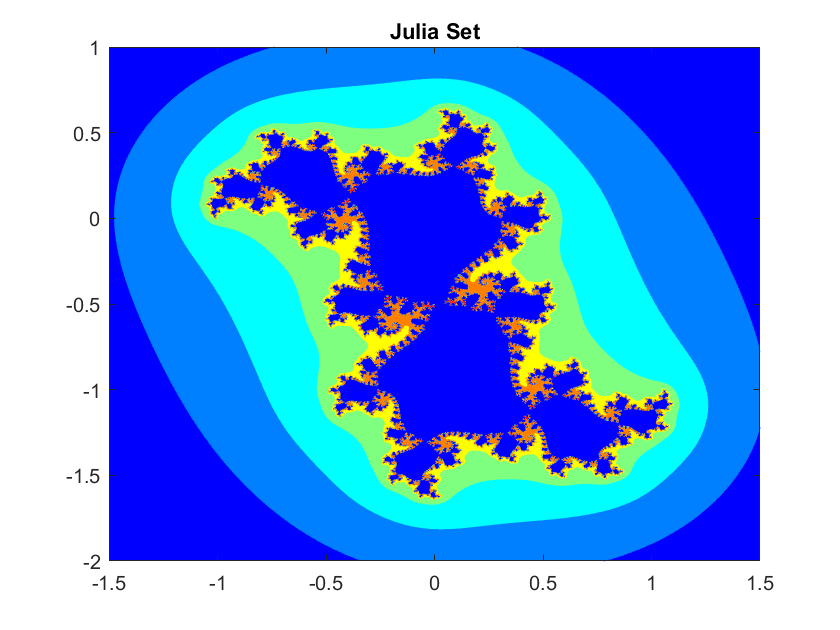
\includegraphics[width=1.2\linewidth]{siegel_julia_set}
%\caption{The Julia set of the dynamical system we are studying with $a = e^{\phi i}$.}
\end{subfigure}
\begin{subfigure}{.5\textwidth}
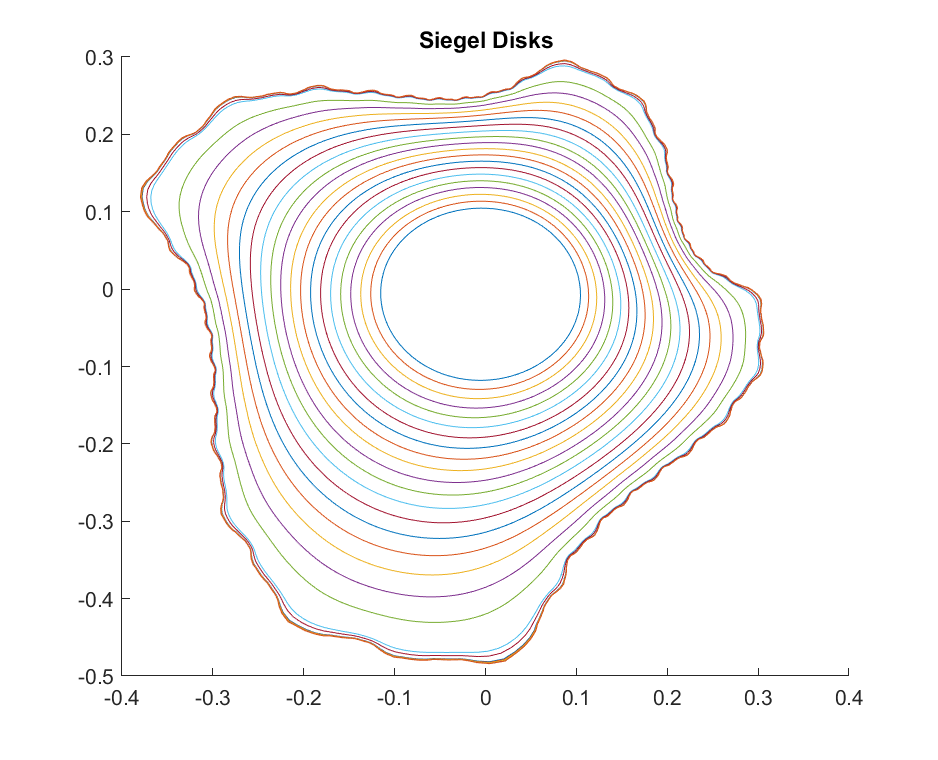
\includegraphics[width=1.1\linewidth]{siegel_disk}
%\caption{Siegel disks output of expanding\_script.m at the time of writing.}
\end{subfigure}
\caption{Visualization of output}
\end{figure}

\noindent
\begin{figure}[h!]
\begin{subfigure}{.5\textwidth}
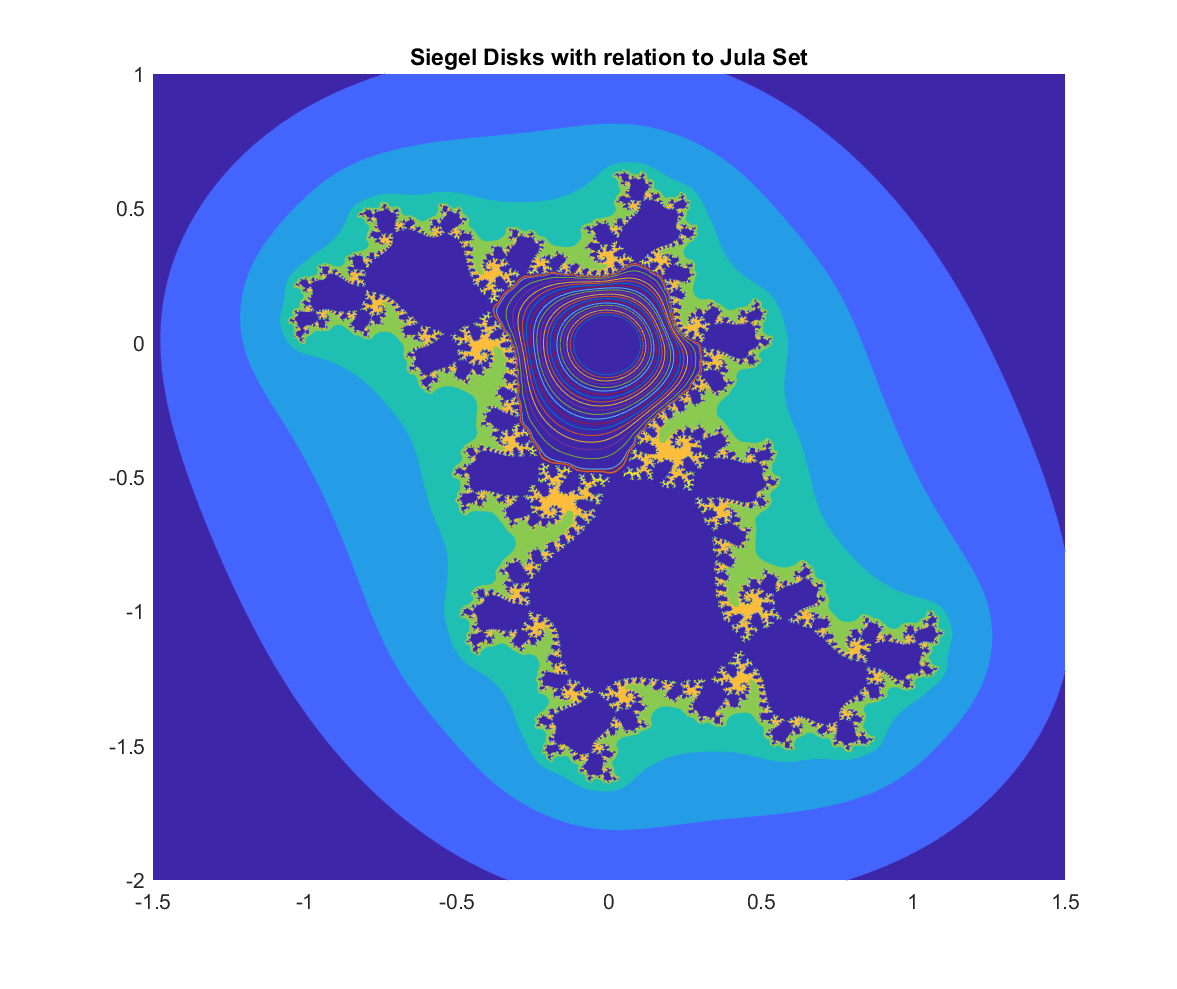
\includegraphics[scale=.35]{siegel_julia_combined}
\end{subfigure}
\begin{subfigure}{.5\textwidth}
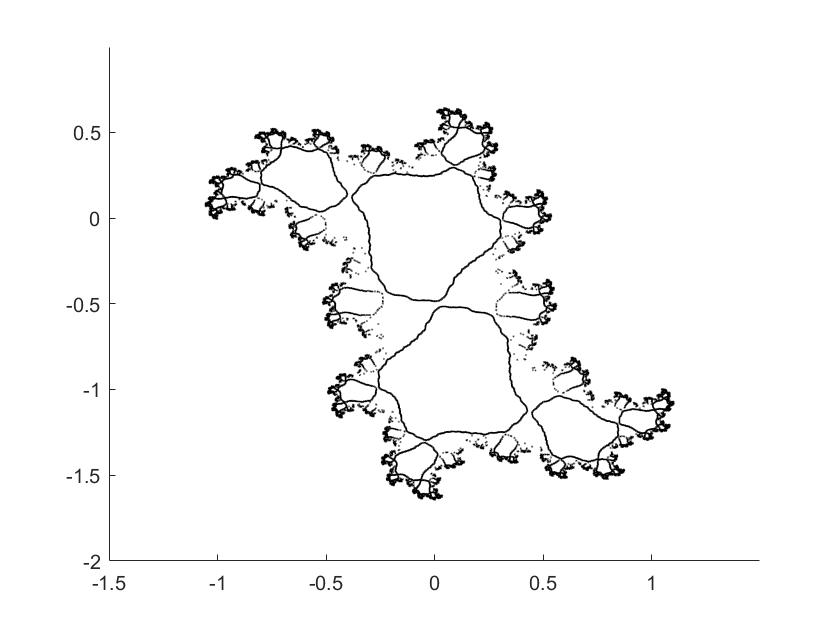
\includegraphics[scale=.27]{preimage_julia_set}
\end{subfigure}
\end{figure}

\subsection{Function Space Information}
\begin{figure}[h!]
\centering
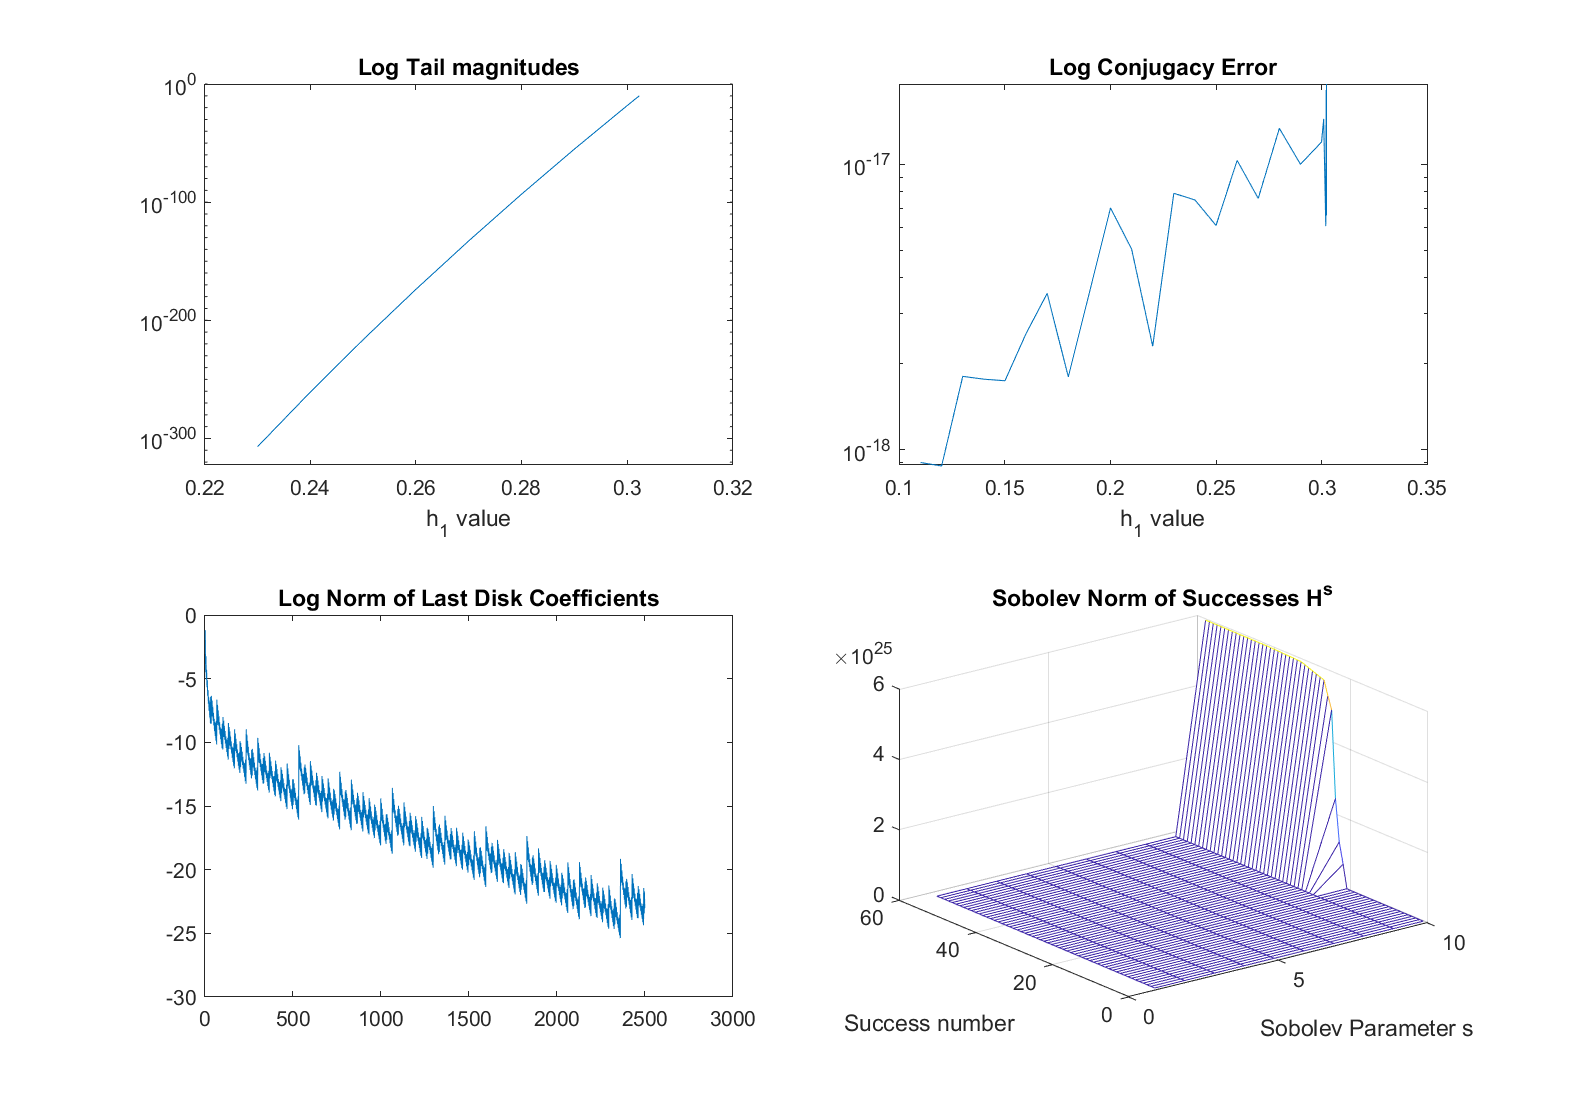
\includegraphics[scale=.4]{siegel_disk_defect}
\caption{Log plot of tail magnitudes and conjugacy error.}
\end{figure}

% \clearpage
\noindent
Number of successful attempts is 58, out of 72 iterations. 

\noindent
Final $\hat{h}_1$ value is 0.302326823002451.

\noindent
Error size on final step 1e-17.

\noindent
Magnitude of last coefficent on last step 1e-10.


\section{Siegel Center Theorem}

This section will be used to prove the Siegel Center theorem, in a couple different formats as a starting point to the preliminary presentation.

I'd like to know a few things about what is going on here...
\begin{itemize}
\item What does the theorem actually say?

An analytic function, under certain assumptions, is analytically conjugate to its linear part on a small-enough neighborhood of the origin. More or less.

\item What sort of problems would be solved by this?
\item What  sort of numbers are actually Diophantine?
\item How does one practically implement the iterative process to compute $h$?
\item How does one compute the Siegel radius?
\item What is the iterative scheme exactly?
\end{itemize}

\begin{theorem}[1 Dimensional Siegel Center Theorem]
Let $U \subset \C$ be a neighborhood of $0 \in \C$, and $f: U \to \C$ be an analytic function of the form,
\begin{equation}
f(z) = az + \hat{f}(z)
\end{equation}
where $\hat{f}(z)$ is $O(z^2)$.

Assume that
\begin{equation}
\left|(a^n - 1)^{-1}\right| \leq n^\nu K
\end{equation}

for some $\nu \geq 1$ and $K > 0$. 
Assume as well that
\begin{equation}
\| \hat{f} \|_1 \leq \rho(\nu) K^2
\end{equation}

where $\rho$ is an explicit function of $\nu$. 

There there exists an unique function
\begin{equation}
h(z) = z + \hat{h}(z)
\end{equation}

with $\hat{h}$ analytic in a disk of radius $\sigma = 1 - 2 \rho(\nu)$ such that 
\begin{equation}
f \circ h(z) = h(az)
\end{equation}

Moreover, 
\begin{equation}
\| \hat{h}\|_\sigma	\leq C \| f \|_1
\end{equation}

\end{theorem}

Questions
\begin{itemize}
\item What are $\| \cdot \|_1$ and $\| \cdot \|_\sigma$? I believe they are sup norms... just have to loop up what is used for analytic functions.

\item What does it mean for a function $\rho(\nu)$ to be an explicit function of $\nu$?
\end{itemize}

\bigskip

We should break down the proof as follows,
\begin{itemize}
\item Basic Outline
\item Difficulties: small divisors, shrinking of domain, smoothness assumptions
\item Technical Lemma
\item Set up function spaces \& Newton-like method
\item Convergence bounds
\item Induction bounds
\item Put it all together
\end{itemize}

\bigskip


\begin{proof}
Sketch:

We can think of 
\begin{align*}
f \circ h(z) = h(az)\\
0 = f \circ h(z) - h(az)
\end{align*}
as an implicit equation in a space of functions, ie as a zero of 
\begin{align*}
\mathcal{T}(f,h) = f \circ h - h \circ a
\end{align*}
Note, $\mathcal{T}(a, Id) = 0$.

Consider a $f$ fixed close to $a$, and an approximate solution $h$ and say,
\begin{align}\label{T=R}
\mathcal{T}\left(f,h\right) = R
\end{align}
for some remainder $R$ which we will think of a small.

We obtain a $\Delta$ that eliminates most of $R$ so $\mathcal{T}\left(f, h + \Delta\right) \ll R$. 
This is a Newton-like method, we start by approximating the correction,
\begin{align*}
\mathcal{T}\left( f , h + \Delta \right) \approx \mathcal{T} \left( f, h \right) + D_2 \mathcal{T} \left( f, h \right) \Delta
\end{align*}
We want 
\begin{align*}
\mathcal{T} \left(f, h + \Delta \right) = 0
\end{align*}
Which can be approximated by using the approximation above,
\begin{align}\label{RD2}
R + D_2 \mathcal{T}\left( f, h \right)\Delta = 0
\end{align}
We can write the derivative,
\begin{align*}
D_2\mathcal{T} \left( f , h \right) \Delta &= \left.\frac{d}{dt}\right|_{t=0}F(f,h+t\Delta) \\
&= \left.\frac{d}{dt}\right|_{t=0} f \circ (h + t\Delta) - (h + t\Delta)\circ a\\
&= \left.\left(\left(f^\prime \circ (h + t\Delta)\right)\Delta - \Delta\circ a \right)\right|_{t = 0}\\
&= \left( f^\prime \circ h \right) \Delta - \Delta \circ a
\end{align*}

So we can substitute this into \ref{RD2},
\begin{align*}
\left( f^\prime \circ h \right) \Delta - \Delta \circ a = - R
\end{align*}
If we could reduce $f^\prime \circ h = a + \hat{f}^\prime \circ h$ was just $a$, this would reduce to that considered in Lemma \ref{lemma-36} (see below). 

Take derivatives wrt $z$ of \ref{T=R},
\begin{align*}
\left( f^\prime \circ h \right) h ^ \prime - a \left( h^\prime \circ a \right) = R^\prime
\end{align*}
Moreover, instead of looking for $\Delta$ directly, we use the fact that $h$ is analytic and near the identity, so we look equivalently for $w$ defined by $\Delta = h^\prime w$. 
The previous equation becomes,
\begin{align*}
\left( f^\prime \circ h \right) h^\prime w - \left( h^\prime \circ a \right)\left( w \circ a\right)  = - R
\end{align*}
Substituting $\left( f^\prime \circ h \right) h ^ \prime = a \left( h^\prime \circ a \right) + R^\prime$ in,
\begin{align*}
a \left( h^\prime \circ a \right) w - \left( h^\prime \circ a\right)\left( w \circ a\right)  = - R - R^\prime w
\end{align*}
We note that $h^\prime$ is of order 1, since $\Delta$ is small, $w$ must be small.
Also $R$ is small, so $R^\prime w$ must be small. 
So we ignore $R^\prime w$. 
Factor and divide
\begin{align}\label{w-eq}
aw - w\circ a = - \left(h^\prime\circ a\right)^{-1} R
\end{align}
This is of the form from Lemma \ref{lemma-36}. 
Therefore we can solve it for $w$, and $\Delta$ in turn.

The proof finishes by the iteration
\begin{enumerate}
\item Take $w$ solving \ref{w-eq}.
\item Form $\Delta = h^\prime w$
\item Then $h + \Delta$ should be a better solution to the problem.
\end{enumerate}
It must be shown that the procedure improves the estimate, as well as the procedure can be repeated infinitely many times and converges to an analytic function.
\end{proof}

Here is the technical lemma referenced in the sketch of proof. 
It was proved in Chapter 2 of KAM Tutorial in a more general format. 
I would like to prove it as stated here...

\begin{lemma}\label{lemma-36}
Assume that $a$ is Diophantine $(K, \nu)$. Then if $\nu(0) = \nu_0 = 0$, we can find a solution of 
\begin{align*}
\varphi(az) - a \varphi(z) = \nu(z); && \varphi(0) = 0
\end{align*}
Moreover,
\begin{align*}
\| \varphi \|_{re^{-\delta}} \leq CK | \delta |^{-\tau} \| \nu \|_r
\end{align*}
where $\tau$ is related to $\nu$ from the Diophantine condition.
\end{lemma}

\begin{proof}

\end{proof}

Here is the lemma showing the convergence of the iteration.

\begin{lemma}\label{lemma-38}
Let $f$ be as in the 1-D Siegel Center Theorem, $h(z) = z + \hat{h}(z)$, $\hat{h}(z) = O(|z|^2)$, defined in a ball of radius $\frac{1}{2} < \sigma < 1$ satisfying
\begin{align*}
\| \hat{h}^\prime \|_\sigma \leq M \leq \frac{1}{2}
\end{align*}
with
\begin{align*}
\sigma + M < 1 \\
\| f \circ h - h \circ a \|_\sigma \leq \varepsilon
\end{align*}
Assume furthermore that $\delta	> 0$ is such that 
\begin{align*}
KC \delta^{-\nu-1}\varepsilon+\sigma e^{-\delta} < \sigma
\end{align*}
Then, the prescription above can be carried out and we have,
\begin{align*}
\| f \circ (h + \Delta) - (h + \Delta)\circ a \|_{\sigma e^{-\delta}} \leq KC \delta^{-\nu-1}\varepsilon^2 + \frac{1}{2} \| f \|_1 (KC \delta^{-\nu-1}\varepsilon M)^2\delta^{-2}
\end{align*}
\end{lemma}

\section{Conclusions}% Probably

\subsection{General Observations}

\begin{remark}
I have noticed that the large steps will fail, however this is not always due to there not being a disk there. Sometimes it s a matter of not having a high enough order. 
\end{remark}

\begin{remark}
It is also worth nothing that the iterative approach is unnecessary in the sense that each guess does not depend in any meaningful way on the previous guesses. 
Therefore, parallel computations could be employed to speed up the process. 
\end{remark}

\subsection{Questions}

\begin{itemize}[noitemsep, topsep=0pt]
\item \st{Is there a norm that we would expect to blow up as we approach the boundary?}

Yes, the sobolev $H^s = W^{s,2}$ norms. 

\item \st{Rafael de la Lave fixes $\hat{h}_1 = 1$ that doesn't seem to lead to a convergent series, any idea why?}

It is better for pen and paper work.

\item \st{Follow up, would the radius of convergence be extremely small?}

Yes, hence having to vary $r$ to be smaller than 1. 
Note, outside the Siegel Disk this this series probably diverges.

\item \st{Better way to visualize coeffs?}

Done. 
\end{itemize}

\subsection{Next Tasks}

\begin{itemize}[noitemsep, topsep=0pt]
\item \st{Try with different $a$, look for other diophantine numbers.} It works well
\item \st{Make a Julia set plotter, pseudo-code available }\href{https://en.wikipedia.org/wiki/Julia_set}{\st{on wikipedia}}.
\item \st{Combine Julia set plot with output} Clean it up some
\item \st{Implement a pre-image plotter} not sure this does anything useful for us.
\item \st{Look over Sobolev spaces and Parseval\'s theorem }\href{https://en.wikipedia.org/wiki/Sobolev_space}{\st{on wikipedia}}\st{ and justify the use.}
\item Add sections about INTLAB as outlined in \cite{Ru99a}. 
First, read \href{http://eprints.maths.manchester.ac.uk/1204/1/narep416.pdf}{this paper} and learn some INTLAB. \cite{intervalanalysis}
\item Try with different $f$, for transcendental $f$ this will require autodifferentiation.
\item \st{Work on single dimensional version of Lemma 2.1} \href{http://cosweb1.fau.edu/~jmirelesjames/preprints/reducibilityPublished.pdf}{in paper}, work on a tail only version $|\alpha| \geq n$ \cite{parampaper}
\item Write section explaining background for above... did some... do more
\end{itemize}

\medskip

\printbibliography
\end{document}